% -*- latex -*-
%%%%%%%%%%%%%%%%%%%%%%%%%%%%%%%%%%%%%%%%%%%%%%%%%%%%%%%%%%%%%%%%
%%%%%%%%%%%%%%%%%%%%%%%%%%%%%%%%%%%%%%%%%%%%%%%%%%%%%%%%%%%%%%%%
%%%%
%%%% This text file is part of the source of 
%%%% 'Parallel techniques'
%%%% by Ángel de Vicente, copyright 2019
%%%%
%%%% TO DO:
%%%%
%%%% barnes-hut-mpi-code.tex : implementation of the Barnes-Hut algorithm in parallel
%%%%
%%%%%%%%%%%%%%%%%%%%%%%%%%%%%%%%%%%%%%%%%%%%%%%%%%%%%%%%%%%%%%%%
%%%%%%%%%%%%%%%%%%%%%%%%%%%%%%%%%%%%%%%%%%%%%%%%%%%%%%%%%%%%%%%%

In order to implement the Barnes-Hut algorithm in parallel, we can have a number
of options. Let's explore two of them.

\begin{enumerate}

\item The first solution we could implement is similar to the parallel version
  not using Barnes-Hut. We can assign to each process a number of bodies for
  which it will be responsible. The tree that we build with the Barnes-Hut
  algorithm can be built by all the processes (or perhaps we could do that only
  one builds it and then sends it to the other processes, but that would be more
  inefficient), and then each process calculates how all the bodies affect the
  particles it is responsible for. This result can then be sent to the other
  processes, so then all processes will have the new updated positions for all
  bodies and then can continue with the {create tree ; calculate forces} loop.

\item The second solution is more efficient, since we can parallelize both the
  forces calculation and the building of the tree. The initial box is divided in
  8 octants (and then later recursively each octant in another 8, etc.), so we
  can implement this solution for 8 processes, where each process will take care
  of one octant. Thus, each process will build a partial tree, for the bodies
  that belong to its octant. When the tree is built, we can calculate how the
  bodies in my tree affect all particles. Then, by using the function
  MPI\_ALLREDUCE we can add up the accelerations for all particles produced by
  the 8 different trees belonging to each of the octants. This solution is
  slightly more difficult than the first one (and meant for a fixed number of
  processes), but we perform in parallel both the forces calculation and the
  tree building, so its performance is much better than solution 1.
\end{itemize}

\Level 0 {Solution 1}
\listing{barnes-hut.parallel.solution1.f90}{chapters/code/barnes-hut.parallel.solution1.f90}

\Level 0 {Solution 2}
\listing{barnes-hut.parallel.solution2.f90}{chapters/code/barnes-hut.parallel.solution2.f90}

\Level 0 {Parallel version performance}

\begin{figure}[!htbp]
  \centering
  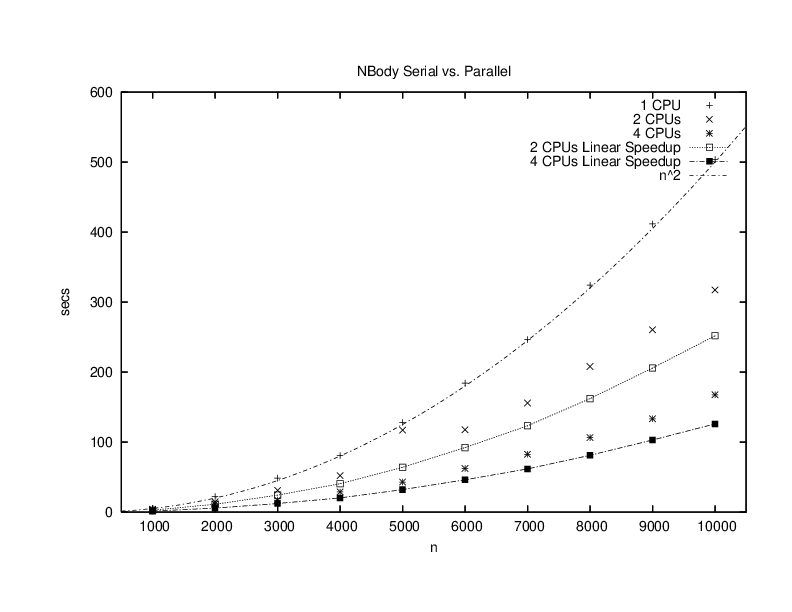
\includegraphics[origin=c,width=0.9\textwidth]{graphics/performance_serial_vs_parallel.png}
  \label{fig:perf-bh-mpi2}
  \caption{Performance Barnes Hut - serial vs. parallel}
\end{figure}


\begin{figure}[!htbp]
  \centering
  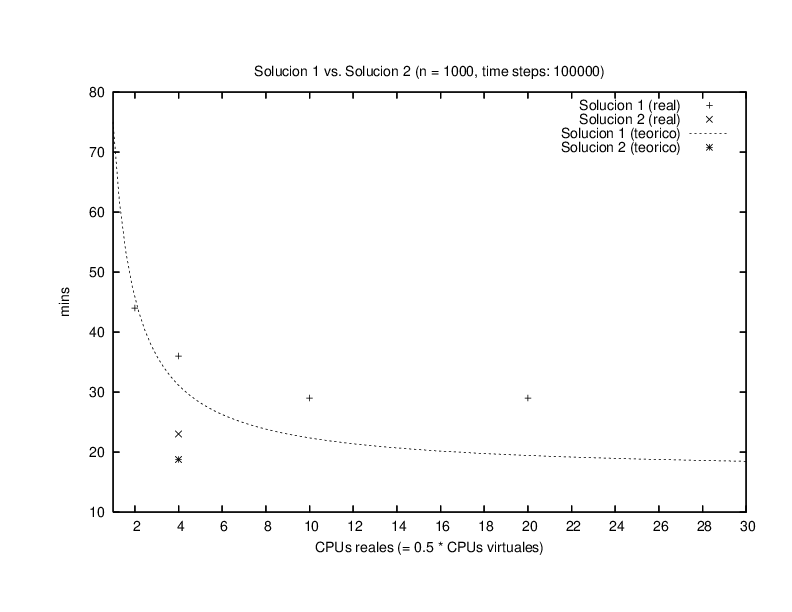
\includegraphics[origin=c,width=0.9\textwidth]{graphics/solution1_vs_solution2.png}
  \label{fig:perf-bh-mpi1}
  \caption{Performance Parallel Barnes Hut - solution 1 vs. solution 2}
\end{figure}




